% Options for packages loaded elsewhere
\PassOptionsToPackage{unicode}{hyperref}
\PassOptionsToPackage{hyphens}{url}
%
\documentclass[
]{book}
\usepackage{amsmath,amssymb}
\usepackage{lmodern}
\usepackage{iftex}
\ifPDFTeX
  \usepackage[T1]{fontenc}
  \usepackage[utf8]{inputenc}
  \usepackage{textcomp} % provide euro and other symbols
\else % if luatex or xetex
  \usepackage{unicode-math}
  \defaultfontfeatures{Scale=MatchLowercase}
  \defaultfontfeatures[\rmfamily]{Ligatures=TeX,Scale=1}
\fi
% Use upquote if available, for straight quotes in verbatim environments
\IfFileExists{upquote.sty}{\usepackage{upquote}}{}
\IfFileExists{microtype.sty}{% use microtype if available
  \usepackage[]{microtype}
  \UseMicrotypeSet[protrusion]{basicmath} % disable protrusion for tt fonts
}{}
\makeatletter
\@ifundefined{KOMAClassName}{% if non-KOMA class
  \IfFileExists{parskip.sty}{%
    \usepackage{parskip}
  }{% else
    \setlength{\parindent}{0pt}
    \setlength{\parskip}{6pt plus 2pt minus 1pt}}
}{% if KOMA class
  \KOMAoptions{parskip=half}}
\makeatother
\usepackage{xcolor}
\IfFileExists{xurl.sty}{\usepackage{xurl}}{} % add URL line breaks if available
\IfFileExists{bookmark.sty}{\usepackage{bookmark}}{\usepackage{hyperref}}
\hypersetup{
  pdftitle={데이터 시각화},
  pdfauthor={한국 R 사용자회},
  hidelinks,
  pdfcreator={LaTeX via pandoc}}
\urlstyle{same} % disable monospaced font for URLs
\usepackage{longtable,booktabs,array}
\usepackage{calc} % for calculating minipage widths
% Correct order of tables after \paragraph or \subparagraph
\usepackage{etoolbox}
\makeatletter
\patchcmd\longtable{\par}{\if@noskipsec\mbox{}\fi\par}{}{}
\makeatother
% Allow footnotes in longtable head/foot
\IfFileExists{footnotehyper.sty}{\usepackage{footnotehyper}}{\usepackage{footnote}}
\makesavenoteenv{longtable}
\usepackage{graphicx}
\makeatletter
\def\maxwidth{\ifdim\Gin@nat@width>\linewidth\linewidth\else\Gin@nat@width\fi}
\def\maxheight{\ifdim\Gin@nat@height>\textheight\textheight\else\Gin@nat@height\fi}
\makeatother
% Scale images if necessary, so that they will not overflow the page
% margins by default, and it is still possible to overwrite the defaults
% using explicit options in \includegraphics[width, height, ...]{}
\setkeys{Gin}{width=\maxwidth,height=\maxheight,keepaspectratio}
% Set default figure placement to htbp
\makeatletter
\def\fps@figure{htbp}
\makeatother
\setlength{\emergencystretch}{3em} % prevent overfull lines
\providecommand{\tightlist}{%
  \setlength{\itemsep}{0pt}\setlength{\parskip}{0pt}}
\setcounter{secnumdepth}{5}
\usepackage{booktabs}
\usepackage{amsthm}
% \usepackage{kotex}

% \usepackage[T1]{fontenc}
% \usepackage[utf8]{inputenc}
%% 한글 폰트
% \setmainhangulfont{MalgunGothic} % NanumMyeongjo
% \setmainhangulfont{NanumMyeongjo} % NanumMyeongjo
% \setsanshangulfont{맑은 고딕}     % MalgunGothic
% \setmonohangulfont{D2Coding}

\makeatletter
\def\thm@space@setup{%
  \thm@preskip=8pt plus 2pt minus 4pt
  \thm@postskip=\thm@preskip
}
\makeatother
\ifLuaTeX
  \usepackage{selnolig}  % disable illegal ligatures
\fi
\usepackage[]{natbib}
\bibliographystyle{apalike}

\title{데이터 시각화}
\author{한국 R 사용자회}
\date{2022-05-03}

\begin{document}
\maketitle

{
\setcounter{tocdepth}{1}
\tableofcontents
}
\hypertarget{uxb370uxc774uxd130-uxc2dcuxac01uxd654}{%
\chapter*{데이터 시각화}\label{uxb370uxc774uxd130-uxc2dcuxac01uxd654}}
\addcontentsline{toc}{chapter}{데이터 시각화}

\begin{center}\rule{0.5\linewidth}{0.5pt}\end{center}

후원계좌

디지털 불평등 해소를 위해 제작중인 오픈 통계패키지 개발과 고품질 콘텐츠 제작에 큰 힘이 됩니다.

\begin{verbatim}
  - 하나은행 448-910057-06204
  - 사단법인 한국알사용자회
\end{verbatim}

\hypertarget{viz-font}{%
\chapter{글꼴}\label{viz-font}}

R을 단순히 통계 언어로 생각하지 말고 적용범위를 확대해서 활용하면
데이터 과학 산출물을 다양한 전자문서로 제작하여 커뮤니케이션 할 수 있다.
PDF, HTML, 워드 등 문서 뿐만 아니라, 파워포인트 같은 발표자료를
슬라이드로 제작하여 배포할 수 있다. 그래프 문법(Grammar of Graphics)에 따라
\texttt{ggplot} 시각화를 산출물에도 다양한 글꼴(font)을 반영하여 좀더 관심을 끌 수 있는
그래프 제작도 가능하다. 데이터 과학자나 개발자 관점에서도 통합개발환경(IDE)이
필요한데 개발과 저작에 집중할 수 있는 글꼴을 지정하여 활용할 경우
생산성도 높일 수 있고 좀더 쾌적한 환경에서 개발을 진행할 수 있다.

R 스크립트 작성을 위한 글꼴과 그래프에 한글 글꼴(font)을 적용한다.
\texttt{ggplot}을 비롯한 시각화를 위해 \texttt{extrafont}와 \texttt{showtext} 패키지를
활용하여 적절한 한글 글꼴을 사용할 뿐만 아니라 코딩 개발할 때
R 스크립트(\texttt{.R}) 및 R마크다운(\texttt{.Rmd})에서도 적절한 한글글꼴 사용을 위해서
코딩관련 글꼴도 설치한다.

기본적인 작업흐름은 운영체제에 먼저 외부에서 가져온 폰트를 설치한다.
그리고 나서 \texttt{extrafont} 팩키지 \texttt{font\_import()} 함수를 사용해서 폰트를
R에서 불러 사용할 수 있도록 설치한다. 그리고 나서 \texttt{loadfonts()} 함수를
사용해서 글꼴을 \texttt{ggplot}등에서 불러 사용한다.
\href{https://fonts.google.com/}{구글 글꼴}을 사용하고자 할 경우 \texttt{showtext} 패키지를
사용해서 로컬 컴퓨터에 설치하여 적용한다.

\begin{figure}
\centering
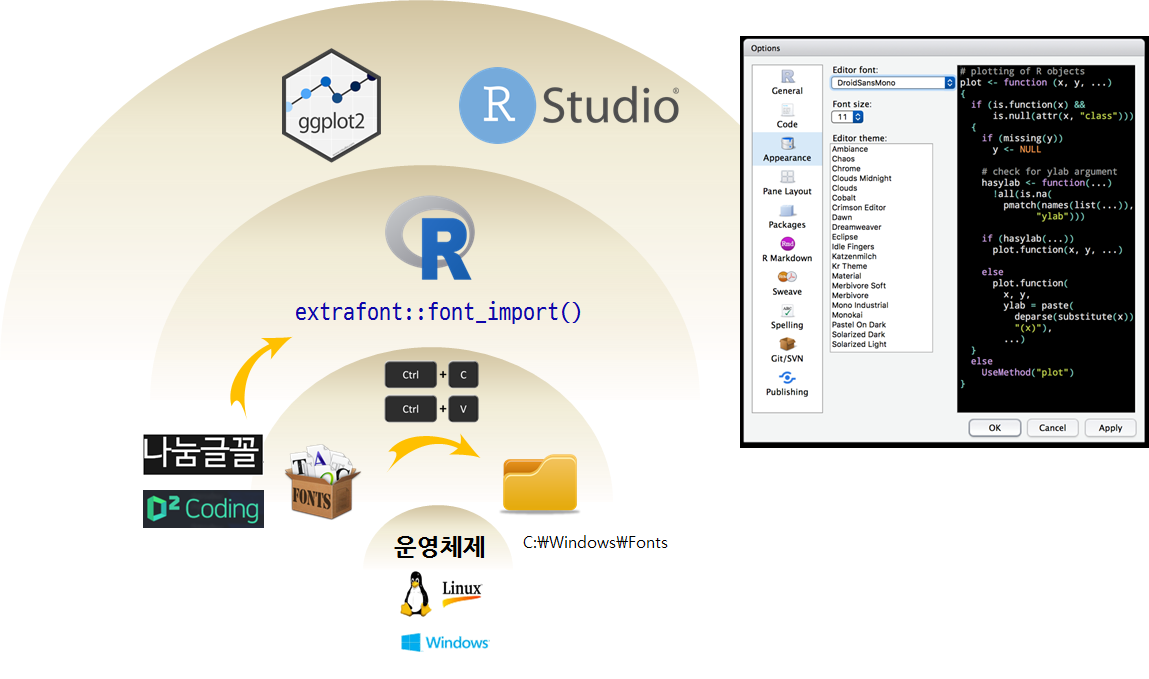
\includegraphics[width=1\textwidth,height=\textheight]{assets/images/font_overview.png}
\caption{R 폰트/글꼴 설치}
\end{figure}

\hypertarget{font-coding}{%
\section{R 코딩 글꼴}\label{font-coding}}

문서를 위해 작성하는데 사용되는 글꼴과 R 코딩을 위해 사용되는 글꼴은
차이가 난다. 왜냐하면 R 코딩에 사용되는 글꼴은 가독성이 좋아야하고
디버깅에 용이해야 된다. 영어는 \texttt{consolas} 글꼴을 많이 사용하는데 무료가
아니다. 그래서 \texttt{consolas}에서 영감을 받은 SIL 오픈 폰트 라이선스를
따르는 \href{https://en.wikipedia.org/wiki/Inconsolata}{Inconsolata}가 R
코딩에 많이 사용되고 있다. 하지만, R코드를 작성할 때 주석을 한글로
달거나 R마크다운 작업을 할 경우 유사한 기능을 하는 한글 글꼴이 필요하다.

\begin{itemize}
\tightlist
\item
  \href{https://github.com/naver/nanumfont/blob/master/README.md}{네이버 나눔고딕 코딩글꼴}
\item
  \href{https://github.com/naver/d2codingfont}{D2 Coding 글꼴}
\end{itemize}

``네이버 나눔고딕 코딩글꼴''과 ``D2 Coding 글꼴''을 설치하고 나서 RStudio
IDE에서 ``Tools'' → ``Global Options\ldots{}''를 클릭하면 ``Options''창에서
\texttt{Appearance}에서 \textbf{Editor font:}에서 설치한 코딩전용 글꼴을 선택하고
\textbf{Editor theme:}도 지정한다.

\begin{figure}
\centering
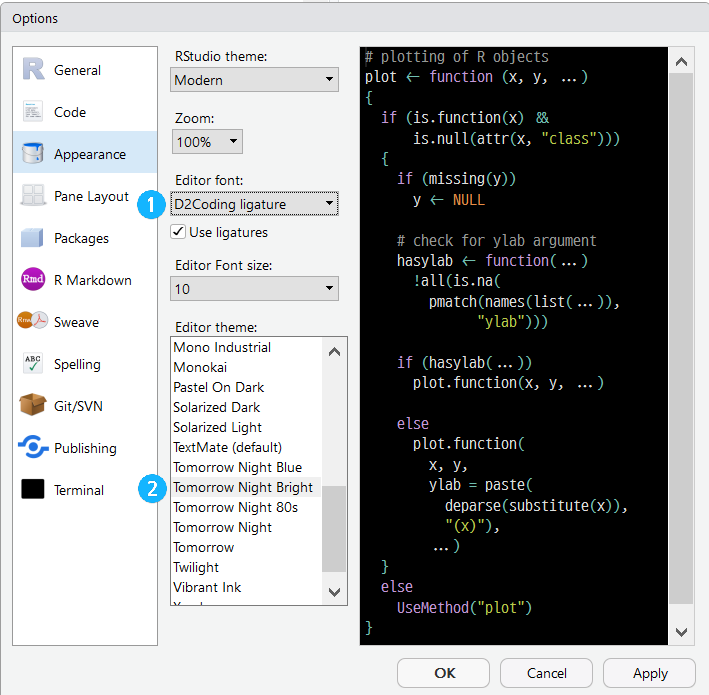
\includegraphics[width=1\textwidth,height=\textheight]{assets/images/font_d2coding.png}
\caption{D2 코딩폰트 설치}
\end{figure}

\hypertarget{r-viz-font}{%
\section{\texorpdfstring{\texttt{ggplot} 시각화 글꼴}{ggplot 시각화 글꼴}}\label{r-viz-font}}

\texttt{extrafont} 팩키지에서 \texttt{font\_import()} 함수로 운영체제(윈도우/리눅스)에
설치된 글꼴을 R로 가져온다. 그리고 나서 \texttt{loadfonts()} 함수를 사용해서
설치된 글꼴을 사용하는 작업흐름을 따르게 된다.

\hypertarget{font-viz-font-example}{%
\subsection{\texorpdfstring{\texttt{ggplot} 한글 글꼴 사례}{ggplot 한글 글꼴 사례}}\label{font-viz-font-example}}

\texttt{extrafont} 패키지 \texttt{loadfonts()} 함수를 사용해서 \texttt{ggplot}에서 적용시킬 수 있는
글꼴을 불러냈다. R 내장 데이터셋 \texttt{iris}를 사용하여 나눔글꼴 ``Nanum Pen Script''을 기본 글꼴로 적용시켰다.

\begin{center}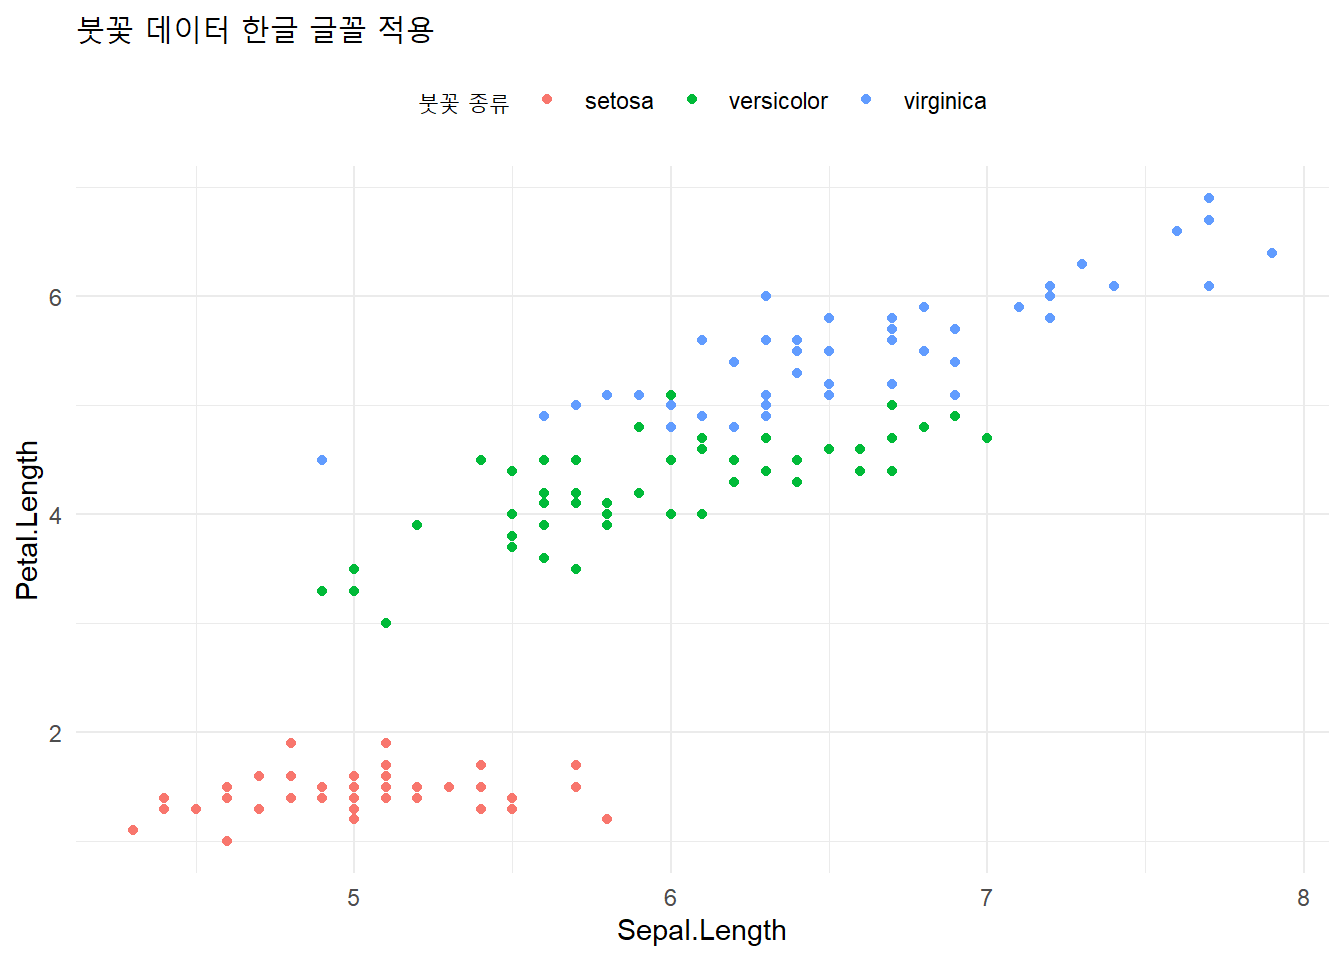
\includegraphics{basics-font_files/figure-latex/ggplot-extrafont-in-r-1} \end{center}

\hypertarget{font-showtext}{%
\section[\texttt{showtext} 패키지 ]{\texorpdfstring{\texttt{showtext} 패키지 \footnote{\href{https://cran.rstudio.com/web/packages/showtext/index.html}{showtext: Using Fonts More Easily in R
  Graphs}}}{showtext 패키지 }}\label{font-showtext}}

\href{https://github.com/wch/extrafont}{extrafont} 패키지를 통해 한자를
포함한 한글을 처리할 수 있었으나, \href{https://github.com/wch/extrafont}{extrafont}는 트루타입폰트(\texttt{.ttf})를
PDF 그래픽 장치에 초점을 맞춰 개발이 되었다. 따라서, 데이터과학
최종산출물이 PDF 형태 책이 아닌 경우 여러가지 면에서 다양한 한글 글꼴을
표현하는데 있어 한계가 있다.

새로 개발된 \href{https://cran.rstudio.com/web/packages/showtext/index.html}{showtext}
팩키지는 \texttt{Ghostscript}같은 외부 소프트웨어를 활용하지 않고도 다양한
(그래픽) 글꼴을 지원한다. \href{https://cran.rstudio.com/web/packages/showtext/index.html}{showtext}로
R 그래프를 생성할 때, 다양한 글꼴(TrueType, OpenType, Type 1, web fonts
등)을 지원한다.

과거 PDF와 같은 책형태로 정보를 공유하고 전달하는 방식이 주류를 이뤘다면
인터넷 등장 이후 웹으로 정보 생성과 소비가 주류로 떠오르게 되면서 글꼴에도
변화가 생겼다. 가까운 미래에는 웹을 우선시하는 글꼴이 대세를 이룰 것으로 보인다.

\begin{figure}
\centering
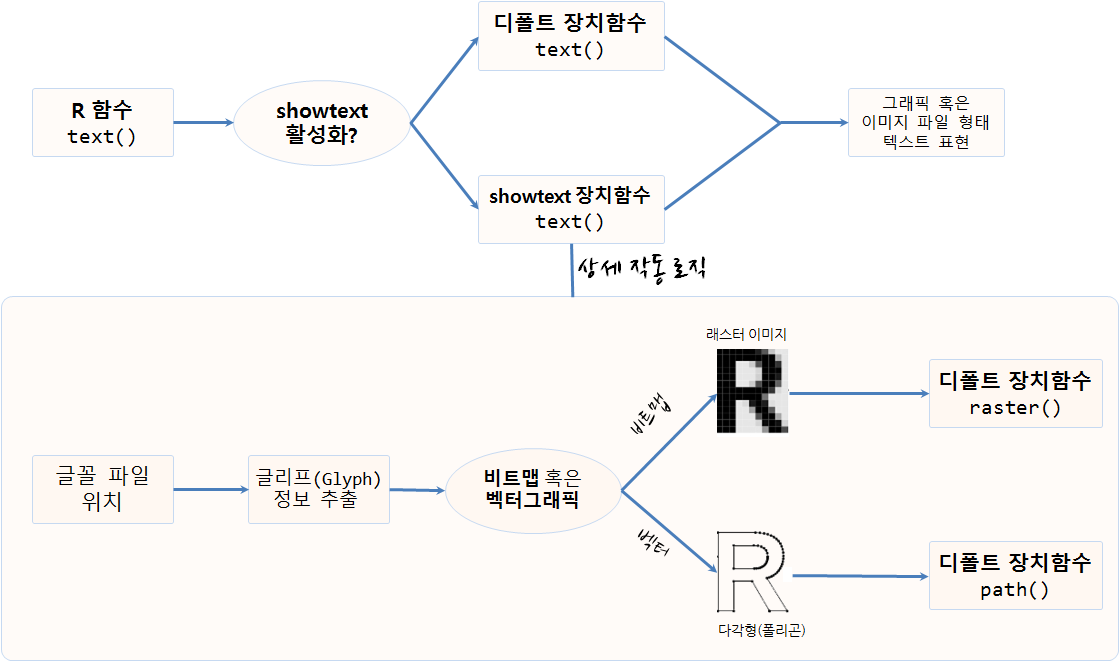
\includegraphics[width=1\textwidth,height=\textheight]{assets/images/font-showtext.png}
\caption{\texttt{showtext} 글꼴}
\end{figure}

사용자가 그래프에 텍스트를 넣기 위해 R 함수에서 \texttt{text()}를 호출할 때
\texttt{showtext}가 활성화 되어 있으면 \texttt{showtext} 팩키지 \texttt{text()} 함수를
호출해서 그래픽 혹은 이미지 파일에 텍스트를 표현하고 그렇지 않는 경우는
디폴트 장치함수 \texttt{text()} 함수를 호출하게 되어 있다.

내부적으로 상세 작동 로직은 글꼴 위치를 파악해서 글리프(glyph) 정보를
추출하고 비트맵 형식, 벡터그래픽 형식에 따라서 비트맵일 경우 \texttt{raster()}
장치함수를 호출하고, 벡터그래픽인 경우 \texttt{path()} 장치함수를 호출해서
기능을 수행한다.

\hypertarget{showtext-korean-example}{%
\subsection{R 설치 글꼴 확인}\label{showtext-korean-example}}

\texttt{extrafont} 팩키지 \texttt{loadfonts()} 함수를 통해 \texttt{.ttf} 파일 정보를
확인한다. 현재 \href{http://www.google.com/fonts}{구글 글끌} 페이지에서 많은 한글
글꼴을 지원하지 않고 있다. 구글에서 전세계 글꼴을 지원하다보 동아시아 3국 대상으로
지원되는 글꼴은 적은 것으로 보인다.

\hypertarget{font-showtext-korean-example-ggplot}{%
\subsection{\texorpdfstring{\texttt{ggplot} 글꼴 적용}{ggplot 글꼴 적용}}\label{font-showtext-korean-example-ggplot}}

한글 글꼴을 바로 적용하기에 앞서 \texttt{showtext} 패키지 포함된 영문글꼴 적용 사례를 먼저 돌려보자.
\texttt{ggplot} 그래픽에 적용되는 \texttt{showtext} 활용 기본 작업흐름은 다음과 같다.

\begin{enumerate}
\def\labelenumi{\arabic{enumi}.}
\tightlist
\item
  글꼴을 적재한다.
\item
  그래픽 장치를 연다
\item
  \texttt{showtext}를 통해 텍스트를 표시한다고 지정한다.
\item
  그래프를 그린다.
\item
  장치를 닫는다.
\end{enumerate}

\hypertarget{font-showtext-korean-example-ttf}{%
\section{로컬 글꼴 적용}\label{font-showtext-korean-example-ttf}}

로컬 컴퓨터에 저장된 \texttt{.ttf} 파일을 사용자 지정해서 가져온 후 이를
\texttt{ggplot}에 반영하여 한글을 R 그래프에 적용하는 것도 가능하다.
\texttt{showtext}는 \texttt{extrafont} 보다 나중에 개발되어 \texttt{extrafont}가
로컬 컴퓨터에 설치된 글꼴을 \texttt{ggplot}에 구현되는데 전력을 다했다면
\texttt{showtext}는 이를 발판으로 나중에 개발되어 구글 폰트와 같은
인터넷 글꼴과 최근 웹출판에 대한 개념도 넣어 개발된 것이 차이점이다.

  \bibliography{book.bib,packages.bib}

\end{document}
